\chapter{Porting of autonomous drive algorithms}
Autonomous driving is a move to the next level driverless transportation. It makes the transportation simpler and easier as the user don’t need to know driving and he doesn't need to apply for a driving license. It sophisticates human living with driverless vehicles and also carries a big set of challenges to the technology. As it is a driverless transportation, maintaining risk-free deals is a typical task. All the autonomous systems works based on the central theme of decision making on input data. Decision making while driving(in the context of autonomous drive systems) without human intervention needs a lot of processing on the huge input data. The autonomous drive system should make a decision real time, thus it gains good control on the vehicle while driving. To make decisions in real time the system should have good hardware support, and all the decision-making algorithms should be implemented efficiently so that they fully utilise the hardware to run in real time. The objective of this chapter is to implement fog rectification, temporal denoising algorithms on embedded R-car H3 SiP platform using multi-core processing and stereo disparity block matching algorithm on NVIDIA GeForce GTX 1070 GPU. 
\section{Embedded automotive platform}
Embedded automotive platforms aim to target the applications in vehicles like In-Vehicle Infotainment (IVI), tracking, object detection, etc. 
\subsection{Rcar-H3 SiP}
Rcar-H3 SiP(System in Package) is announced by Renesas and is not in full production. It is a successor to its previous drive platform Rcar-H2. The Rcar-H3 is fully designed to work for autonomous drive systems. This can be used in vehicles for In-Vehicle Infotainment(IVI), navigation, object detection, collision estimation, etc. The full hardware details of Rcar-H3 SiP are exposed in the Figure \ref{fig:Rcar-H3}.
\subsubsection{Hardware specifications} 
The Rcar-H3 SiP contains a CPU core with ARM®Cortex®-A57 Quad, ARM®Cortex®-A53 Quad and ARM®Cortex®-R7 Dual lock-step. The A-57 is a powerful CPU core while A-53 is little low when compared to A-57. This combination of high and low CPU cores makes ARM’s big.Little architecture. In this architecture, the statements to execute will be streamlined to different cores according to their complexity. The SiP has an external LPDDR4-SDRAM support that will be used to extend the RAM. It has several Audio, video modules which are specifically designed to perform a defined set of functionalities.
\begin{figure}[h!]
	\centering
	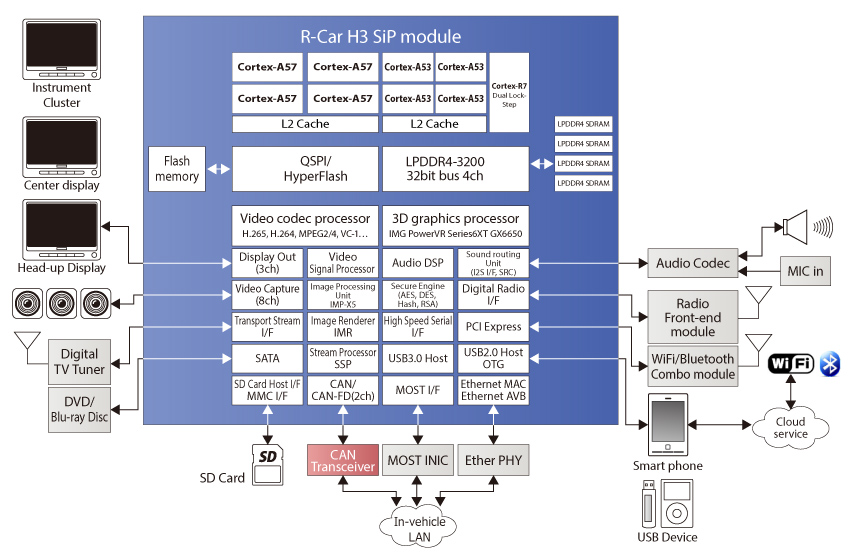
\includegraphics[width=0.9\linewidth]{Rcar-H3.png}
	\caption{Rcar-H3 SiP Hardware block diagram \cite{rcar}}
	\label{fig:Rcar-H3}
\end{figure}
\subsection{Tegra X1 SoC}
Tegra X1 SoC is brought by NVIDIA to compete in the mobile processor line.This SoC contains ARM A-57 quad MPcore  CPU and a Maxwell architecture NVIDIA GPU with 256 cores. It contains special video decoders such as H.265, H.264 for rendering HD, UHD, 4K videos.
\section{Temporal denoising }
The temporal denoising removes the noise between the video frames. It is used in conjunction with other image processing algorithms, like fog rectification, low light enhancement, etc. This algorithm is used in this work to remove the noise component added during the processing of autonomous drive algorithms. This algorithm is implemented on Rcar-H3 SiP using multi-core proessing techniques.
\subsection{Algorithm flow}
In the following, the algorithm flow of Temporal denoising is explained with references. In this work, high performance implementation of this algorithm is designed to get best performance using multi-core CPU computing.
The algorithm is organised into two parts, a) calculating the average frame and b) reconstructing the entire denoised image. The algorithm is shown in the Figure \ref{fig:temporal denoising}. 
\paragraph*{}To describe the algorithm, An average frame($F_a$) is found using the motion of the frames($Pr$) and a current frame($F_c$) as in Equation \ref{average frame}. the average frame is given as, 
\begin{equation}\label{average frame}
F_a = Pr \times F_c + (1-Pr)\times (0.9 \times F_a + 0.1 \times F_c)
\end{equation}
\paragraph*{} The denoised image$F_o$ can be reconstructed as,
\begin{equation}\label{denoised image}
F_o = Pr \times F_c + (1-Pr)\times  F_a
\end{equation}
\begin{figure}[h!]
	\centering
	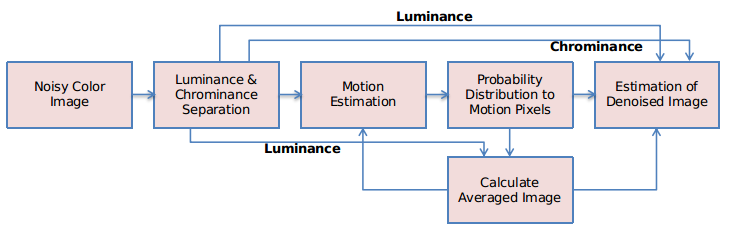
\includegraphics[width=\linewidth]{temporal-denoising.png}
	\caption{block-diagram of temporal denoising algorithm}
	\label{fig:temporal denoising}
\end{figure}
\subsection{Multi-core CPU implementation}
In the initial implementation of the algorithm, entire image was processing on a single core of quad ARM A-57 MPcore in Rar-H3 SiP.  Since a single core contains limited resources and processing an entire image has given less timing performance of the algorithm. To utilise the processing power of all cores, the image is divided and is distributed to process on the four cores in parallel. This ensures the data level parallelism, every core processes a quarter of an image, thus all the four cores will be busy in processing a single image. At the end, the output of all the cores is joined as a single output image.\paragraph*{}The ARM A-57 MPcore is programmed using \textit{pthreads} library to accommodate multi threaading on CPU. Since four cores are available, four threads are created and are mapped to each core. Each thread process quarter of an image by fully utilising hardware resources in it's mapped core. All the threads are run in parallel and the processing of entire image takes less time when compared with the single core implementation.
\subsection{Results and discussions}
The temporal denoising algorithm is implemented on Rcar-H3 SiP embedded platform. The initial implementation of the algorithm runs at 4 FPS, while the multi-core implementation runs at 14.71 FPS on the Rcar-H3 multi-core CPU. The timing performance is shown in the Table \ref{table:Temporal denoising}. The Figure \ref{fig:fog rectification results} shows the input and output to the temporal denoising algorithm. From the table, it is observed that the multi-core implementation is far more better than the single core implementation. It uses the ideal CPU cores and saves considerable power by decreasing execution time.
\begin{figure}[h!]
	\centering
	\subfloat[input]{{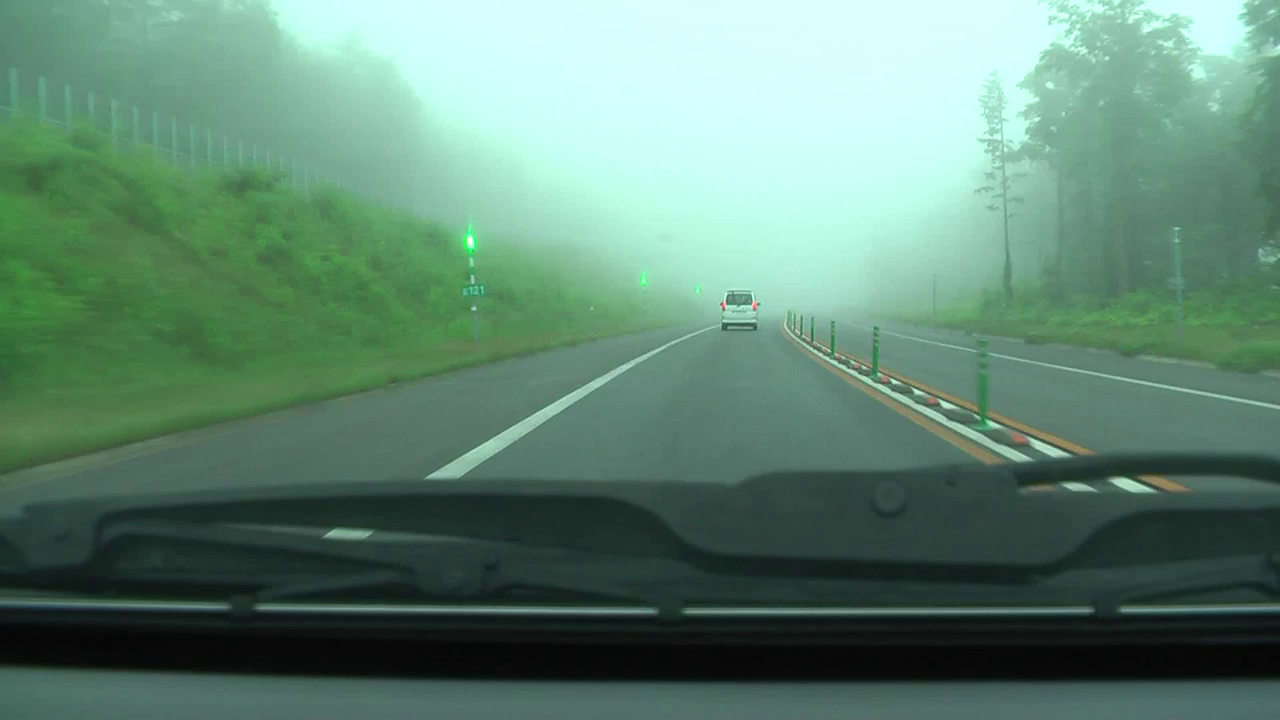
\includegraphics[width=6cm]{tempinput.png} }}%
	\qquad
	\subfloat[output]{{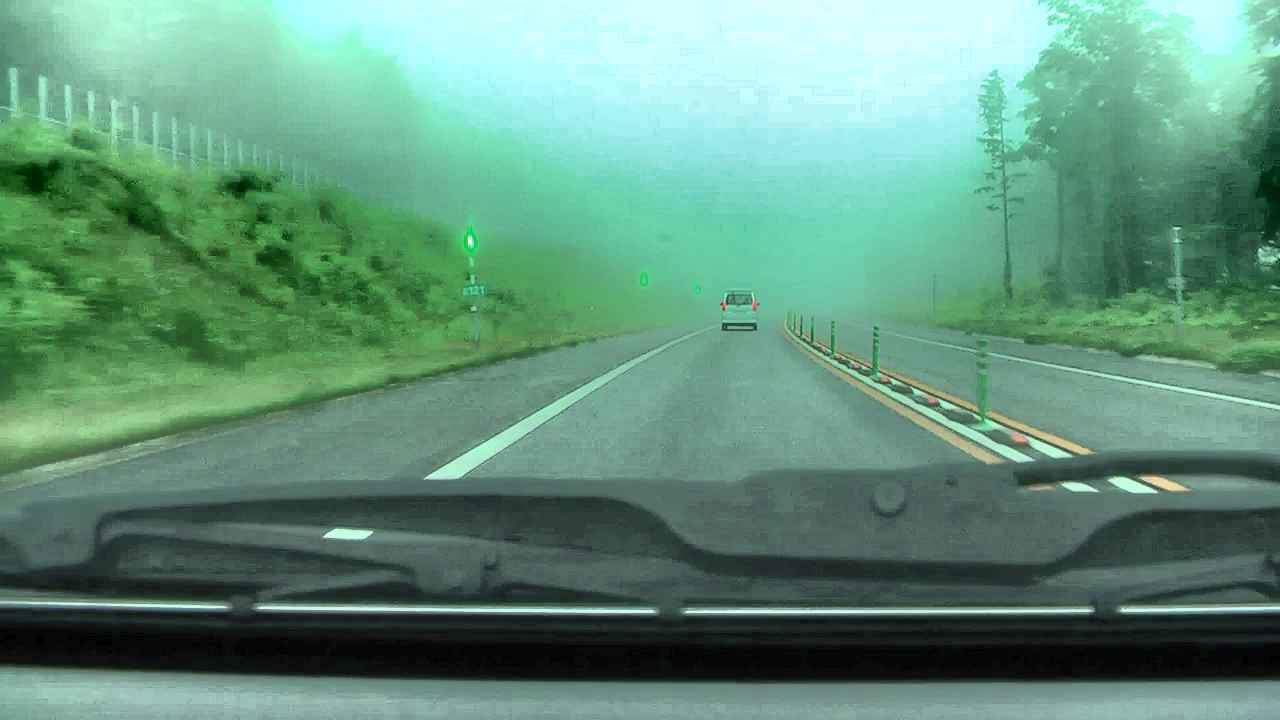
\includegraphics[width=6cm]{tempoutput.png} }}%
	\caption{Temporal denoising algorithm results for an image of size 533x640  }%
	\label{fig:fog rectification results}%og
\end{figure}

\begin{table}[h!]
	\centering
	\resizebox{\columnwidth}{!}{%
	\begin{tabular}{|c|c|c|c|}
	\hline
	\textbf{S.No} &\textbf{Resolution}&\multicolumn{2}{c|}{\textbf{FPS}} \\ \cline{3-4}
	&&\textbf{Without multi-threading}&\textbf{With multi-threading} \\ \hline
	1&600x404&4.5&14.71 \\ \hline
	\end{tabular}}
	\caption{Temporal denoising performance statistics}
	\label{table:Temporal denoising}
\end{table}
\section{Fog rectification with denoising \cite{anisotropic} \cite{dehaze} \cite{fastvis}}
Fog rectification is used to remove the fog from fog affected scenes. It is very useful in autonomous driving in winter seasons, where the information in the scenes is blocked by fog. The fog rectified image may contain noise, thus applying denoising algorithm on the the fog rectified image preserves good details.
\subsection{Algorithm flow}
In the following, the algorithm flow of Fog Rectification is explained with references. In this work, high performance implementation of this algorithm is designed to get best performance using MultiCore CPU computing.
\begin{itemize}
\item Model of fog effect according to Koschmieder law \cite{fogRemoval} \cite{dehaze} \cite{fastvis} \cite{ChrFramework} is given as,
\begin{equation}\label{fog model}
I(x,y)=I_0(x,y)\exp^{-kd(x,y)} + I_\infty(1-\exp^{-kd(x,y)})
\end{equation}
$I(x,y)$ is the observed image intensity at (x,y)
$I_0(x,y)$ is the image intensity without fog at (x,y)
$I_\infty$ is the sky intensity or global atmosperic constant

\item In Equation \ref{fog model}, first term represents the airlight and the other term is direct attenuation. The Equation \ref{fog model} can be re written as Equation \ref{airlight} \cite{fogRemoval}. 
\begin{equation}\label{airlight}
I(x,y)=I_0(x,y) (1-\frac{A(x,y)}{I_\infty})+A(x,y)
\end{equation}
where $A(x,y)$ is the airlight component. 
If $I_\infty \approx 1$ then Equation \ref{airlight} can be modified as,
\begin{equation}\label{airlightmod}
I(x,y)=I_0(x,y) (1-A(x,y))+A(x,y)
\end{equation}
\item The airlight can be estimated using Equation \ref{airlight}. This initial airlight map($A_0(x,y)$) is assumed as Equation \ref{airlight map assumption} \cite{fogRemoval}.
\begin{equation}\label{airlightest}
A(x,y) = \min_{c \in (r,g,b)} (I^c(x,y))-\min_{c \in (r,g,b)}\begin{bmatrix}
{I_0}^c(x,y)(1-\frac{A(x,y)}{I_\infty})
\end{bmatrix}
\end{equation}
\begin{equation}\label{airlight map assumption}
A_0(x,y)=\beta \min_{c\in (r,g,b)}(I^c(x,y))
\end{equation} 
where $\beta$ is a constant and varies between $0<\beta<1$
\item The effect of airlight is different for different objects from camera, since it is a function of distance from camera. So, the airlight effect resembles the anisotropic diffusion \cite{fogRemoval} \cite{anisotropic}.
Anisotropic diffusion is given as,
\begin{align}\label{anisotropiceq}
\frac{\partial A}{\partial t} &= div(\alpha(x,y,t)\nabla A)\\
& = \alpha(x,y,t)\Delta A + \nabla \alpha \nabla A
\end{align}  
where $\alpha$ is the conduction coefficient.
$\Delta$ is the laplacian operator
$\nabla$ is the gradient operator
if $\alpha(x,y,t)$ is constant over space and time then the Equation \ref{anisotropiceq} reduces to the heat diffusion equation as Equation \ref{anisotropicmodeq} explained in \cite{fogRemoval}.
\begin{equation}\label{anisotropicmodeq}
\frac{\partial A}{\partial t} = \alpha \Delta A
\end{equation}
\item According to \cite{fogRemoval} the value of $\alpha$ should be 1 at the interior regions and 0 at the edges. If $E(x,y,t)$ is the expectation of boundaries then the conduction coefficient is given by the Equation  \cite{anisotropic} as,
\begin{equation}\label{condeq}
\alpha=g(|| E ||)
\end{equation}   
where $g(|| E ||)=\exp^{-(\frac{||E||}{k})^2}$, $k$ is a positive constant which is fixed \cite{fogRemoval}.
\item The airlight map can be estimated iteratively using Equation \ref{anisotropiceq} \cite{anisotropic}
\begin{equation}\label{airlight iter est eq}
A^{t+1}=A^t+\lambda \begin{bmatrix}
\alpha \nabla A^t
\end{bmatrix}
\end{equation}
\item The discrete version of the Equation \ref{airlight iter est eq} is,
\begin{equation}\label{discrete airlight est}
\begin{split}
A(x,y,t+1) = & A(x,y,t) + \lambda 
[\alpha_N(x,y,t) \nabla_N A(x,y,t) \\&+ \alpha_S(x,y,t) \nabla_S A(x,y,t) \\&+ \alpha_E(x,y,t) \nabla_E A(x,y,t) \\ &+ \alpha_W(x,y,t) \nabla_W A(x,y,t)]
\end{split}
\end{equation}
The parameter ($\lambda$) is a smoothing parameter and varies as $0<\lambda<1$, $N,S,E$ and $ W$ are subscripts for North, South, East and West.
		\item Once the airlight map $A$ is estimated then de-foggy image is given as,
		\begin{equation}
		I_0(x,y,c)=\frac{(I(x,y,c)-A(x,y))}{(1-(\frac{A(x,y)}{I_\infty(c)}))}
		\end{equation}
		where, $I_0(x,y,c)$ is the de-foggy image,$c\in (r,g,b)$
\end{itemize}
\begin{figure}[h!]
	\centering
	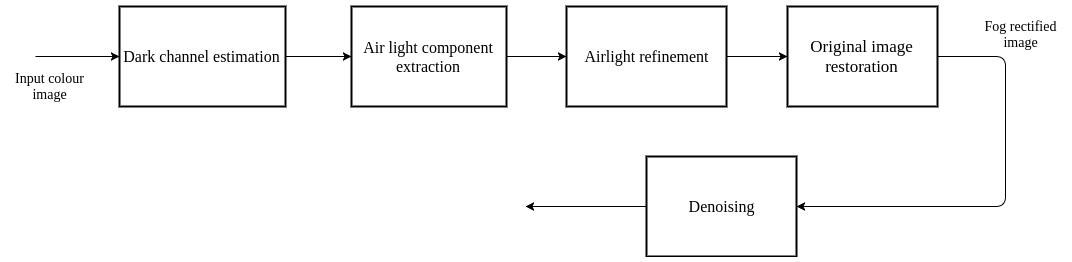
\includegraphics[width=\linewidth]{fogRectWithDenoise.png}
	\caption{Block-diagram of fog rectification with denoising algorithm}
	\label{fig:fog rectification algorithm}
\end{figure}
\subsection{Multi-core CPU implementation}
The single core implementation of fog rectification algorithm takes considerable amount of time to run. The Fog rectification algorithm when implemented on Rcar-H3 SiP embedded hardware is divided into three parts, a)decoding the image, b)processing the image (implement algorithm on the image), and c) displaying the output. In a single core implementation all these portions run on single core, due to the limited resources the execution of these portions will take more time than expected. Thus, processing these three portions of the algorithm in parallel by utilising the all four cores of A57 CPU will improve the timing performance. \paragraph*{} Here, All the three portion of the algorithm are dependent on each other, A direct parallel implementation is not possible. A basic core level pipelining concept is used here. Initially an image is decoded at the processing stage. When the processing stage takes the image for processing then it notifies to decoder to decode a frame. While the processing stage processes the image the decoder on the other hand decodes the image in parallel.  After the completion of processing, the display stage takes the image and notifies the processing stage to process next image, while displaying the previous image, the processing stage processes the next image. This activity goes on, and after few cycles all the three stages will run concurrently but on different images. This methodology is shown in Figure \ref{fig:Parallelism through pipelining}.\paragraph*{} To realize the above methodology we depend on pthreads library for creating threads and semaphore library for ensuring communication among threads. Figure \ref{fig:multi-threading} shows the approach to the multi-threading on multi-core CPU using \textit{pthreads} and \textit{semaphores}.
\begin{figure}[htb]
	\centering
	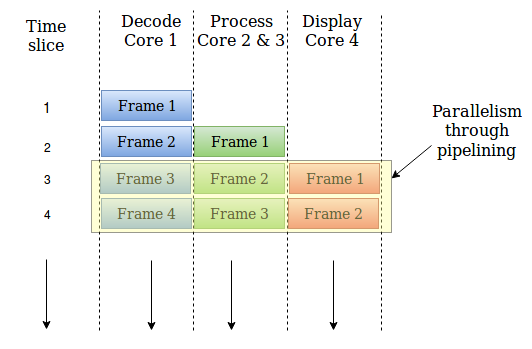
\includegraphics[width=0.8\linewidth]{corelevelpipeline.png}
	\caption{Parallelism through pipelining in fog rectification algorithm}
	\label{fig:Parallelism through pipelining}
\end{figure}%
\begin{figure}[h!]
	\centering
	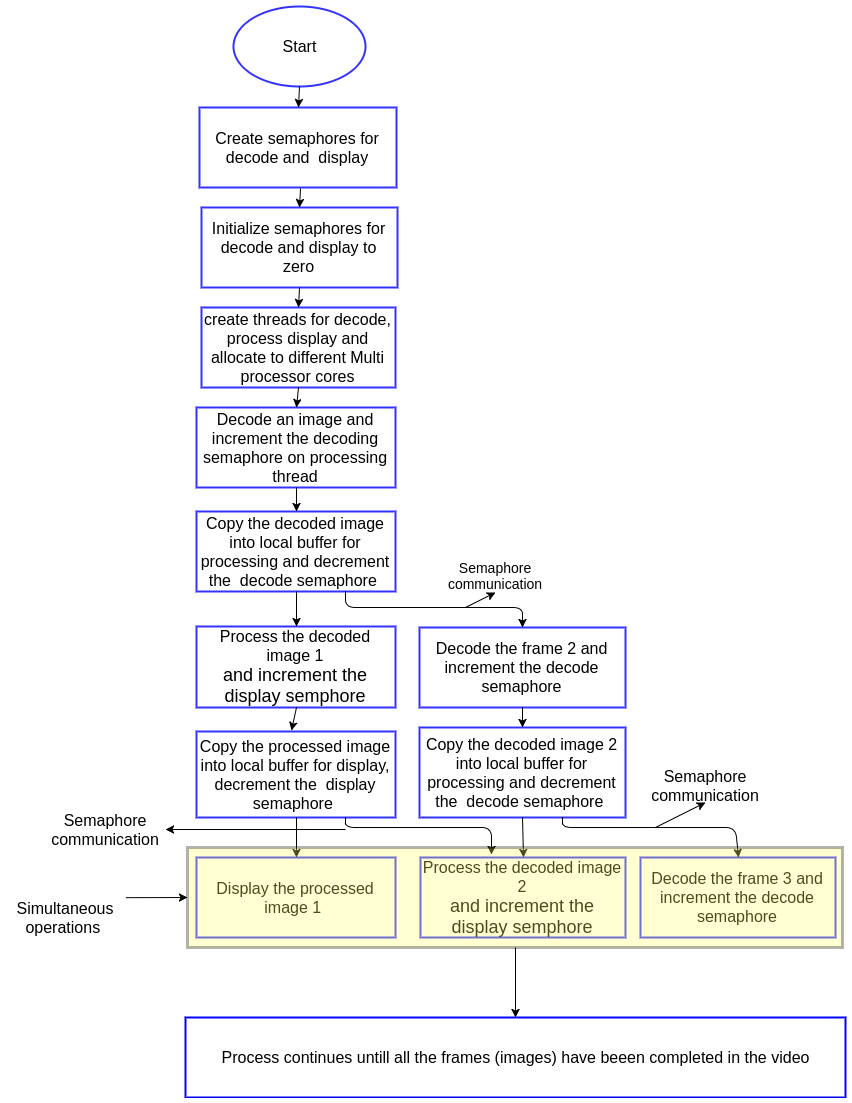
\includegraphics[width=\linewidth]{MPcorePthreads.png}
	\caption{Multi-threading process flow for pipelining on multi-core CPU}
	\label{fig:multi-threading}
\end{figure}%
\paragraph*{}The available hardware in this work is Rcar-H3 which has an active ARM A-57, the decoding part of the algorithm is made to run on the core 1, the Processing part is provided with 2,3 cores, and finally the display part of the algorithm runs on core 4. 
\subsection{Results and discussions}
The fog rectification with denoising is implemented on Embedded hardware Rcar-H3 SiP. This SiP has a quad ARM A57 MPcore CPU. The single core fog rectification with denoising runs at 4 FPS, whereas the multi-core implementation runs at 8 FPS. The results can be seen in the Figure \ref{fig:Fog rectification results} and the timing performance is tabulated in Table \ref{table:fog rectification}.
\begin{figure}[htb]
	\centering
	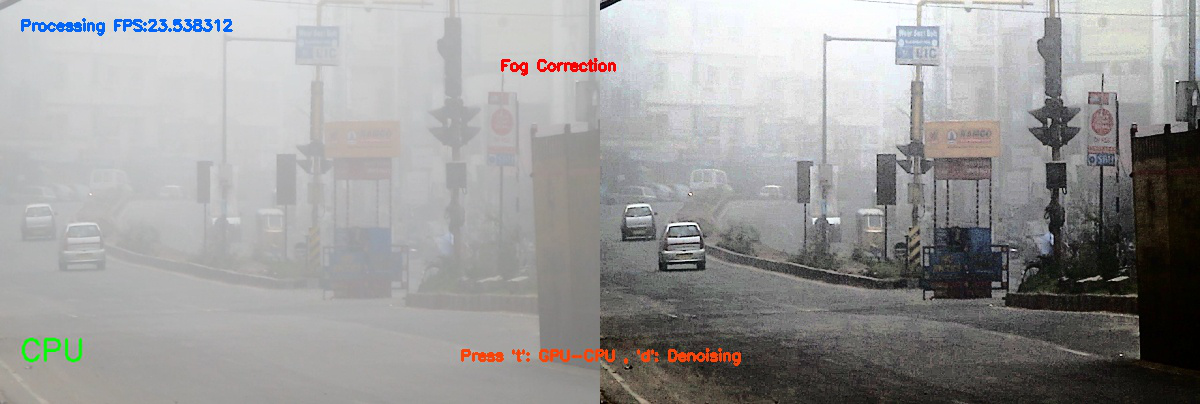
\includegraphics[width=\linewidth]{fogRectresults.png}
	\caption{Fog rectification functional results}
	\label{fig:Fog rectification results}
\end{figure}
From the Table \ref{table:fog rectification}, it is observed that multi-core pipeling implementation of the algorithm performs better than the single core implementation. However, the fog rectification with denoising  has low performance. This is due to the fact that the denoising part uses most of the CPU resources.
\begin{table}[htb]
	\resizebox{\columnwidth}{!}{%
	\begin{tabular}{|c|c|L|L|L|L|}
		\hline
	\textbf{S.No}&\textbf{Resolution}&\multicolumn{4}{c|}{\textbf{FPS}} \\ \hline
	&&\multicolumn{2}{c|}{\textbf{Without denoising}}& \multicolumn{2}{c|}{\textbf{With denoising}} \\ \cline{3-6}
	&&\scriptsize  \textbf{Normal implementation}&\scriptsize  \textbf{Multi-core implementation}&\scriptsize  \textbf{Normal implementation}&\scriptsize  \textbf{Multi-core implementation} \\ \hline
	1&600x404&16&23&4&8.5\\ \hline
\end{tabular}}
\caption{Fog rectification algorithm timing performance}
\label{table:fog rectification}
\end{table}
\section{ Stereo disparity block matching algorithm}
Stereo disparity algorithm is used in 3D image reconstruction by providing the depth of the objects in the image. Stereo disparity works on rectified stereo images, and it produces a disparity map, this disparity map is inversely proportional to the depth map of objects in the image. In autonomous vehicles, it helps in finding the distance of the objects from the vehicle. Stereo disparity two implementations at algorithm level, a) block matching and b) semi global block matching. In this work stereo disparity with block matching implementation is considered.
\begin{figure}[htb]
	\centering
	\includegraphics[width=0.75\linewidth]{stereoDisparityalgorithm.png}
	\caption{stereo disparity block matching algorithm, for 17 disparity levels and a block size of 17x17}
	\label{stereoDisparityalgorithm}
\end{figure}

\subsection{Algorithm flow}
In the following, the algorithm flow of Stereo disparity block matching is explained with references. In this work, high performance implementation of this algorithm is designed to get best performance using GPGPU computing.
\begin{itemize}
	\item Stereo disparity block matching(SBM) works on rectified stereo image pair, one of the pair act as a reference image. In this case right image is taken reference image.
	\item Disparity map is finding the level of similarity in the stereo images. For finding the similarity in the images, a block of pixels is considered instead of single pixel. In this work, the block considered is 17x17.
	\item A block of 17x17 pixels is used in the left image for finding similarity in the reference image over a search window of 16 pixels.
	\item Sum of absolute differences(SAD) matrix is found between the pixel window of left image and reference image, depicted in Equation \ref{SADeq}. And the pixel window in the reference image is shifted by a pixel and a SAD matrix is formed again. This continues upto 16 shifts(disparity levels) in the reference pixel window. This operation is shown in Figure \ref{stereoDisparityalgorithm}.
	\begin{equation}\label{SADeq}
	S_d(x,y) = \sum_{k=1}^{3}\sum_{i=-r}^{r} \sum_{j=-r}^{r} |f(x-i,y-j,k)-g(x-i-d,y-j-d,k)|
	\end{equation}
	where,\\
	$S_d(x,y)$ is SAD cost at $d$ disparity level(pixel shift) for pixel at (x,y)\\
	$d={1,2,....,D}$, $D$ is the maximum number of disparity levels \\
	$r$ is the radius of the window
	and $k$ represents the colour components ($R,G,B$) in the image
	
	\item The shift location($d$) of minimum SAD cost is noted as the disparity value at that pixel.
\end{itemize}
\subsection{Parallel GPU streams implementation}
\begin{itemize}
	\item From the SAD operation, for every SAD value the difference values needed are already available except at that pixel. 
	\item Finding difference between each pixel of both images is sufficient rather using a window based approach. After difference matrix is formed, summing a window of 17x17 elements centered around a pixel in the difference matrix gives the SAD value at that pixel, and it is equivalent to the operation in Equation \ref{SADeq}.
	\item The summation operation to form a SAD matrix is implemented using convolution operation with a 17x17 all 1's kernel. Further this kernel is splited into two linear vectors (horizontal and vertical) with a size of 17 to replace the single 2D convolution with two linear 1D convolutions which is called a separable convolution.
	\item The difference matrix is first operated with the horizontal kernel and later the output is operated with a vertical kernel, this gives the entire 2D convolution output.
	\item This difference matrix is found for 16 times, each time finding difference matrix with a pixel shift in the reference image and SAD matrix is also found with separable convolution.
	\item The shift location of The minimum SAD value among all the SAD matrices gives the disparity value at that pixel (all the SAD values are mapped to respected pixel locations).
	\item The difference operation is performed on all the 3 components (RGB) in a pixel and accumulated to a single value. In GPU, if each output data element is expected to produce by a thread then a data size number of threads will give the entire difference matrix. For an image of size 533x640, a linear grid of 704 blocks with 32x32 threads in each block are created to perform the operation.
	\item The horizontal separable convolution operation is applied on the difference matrix, since the single convolution output uses multiple input data elements so there is a chance of redundant memory transactions. To avoid these unnecessary memory accesses, the difference matrix can be stored in a shared memory and is available to access multiple times with less time cost. To implement this operation in GPU, a 18x20(columnsxrows) 2D grid of blocks is used with 32x32 threads in each block.
	\item So the above methodology implements convolution operation very effectively that it takes very less time compared to the standard implementation. This methodology is used for the other separable convolution too.
	\item The horizontal convolution output is given to vertical separable convolution, the output of vertical convolution gives the SAD matrix. To perform this operation in GPU, a 17x20 2D grid of blocks is created with 32x32 threads in each block.
	\item The SAD matrix is compared against with the previous minimum SAD values stored in a matrix, and minimum is placed in the minimum SAD value matrix and shift location of minimum SAD value is also stored in a disparity matrix. This operation runs on a GPU kernel with 667 linear blocks, each block is having 512 threads.
	\item Texture Memory can be used in the above algorithm for containing image, it makes fast accessing of image data. \hfill \break
	\begin{itemize}
		\item From the above CUDA kernel which performs difference operation, it is evident that there is a possibility to increase speed up using texture memory.
		\item NVIDIA provides for its GPU a special cache called texture memory for 2D locality referencing. The memory costs are very less when a variable is read from texture cache. The texture memory is read only.
		\item  As shown in the Figure \ref{fig:Texture}, the images can be stored in texture memory.And when a texture element is fetched a 2D element chunk is loaded into cache. The texture memory usage is dominant in window based operations on images. In this case, a block of 17x17 elements can be fetched to cache with a single global memory cost using texture memory. This is technique is not implemented in this work.
			\begin{figure}[h!]
				\centering
				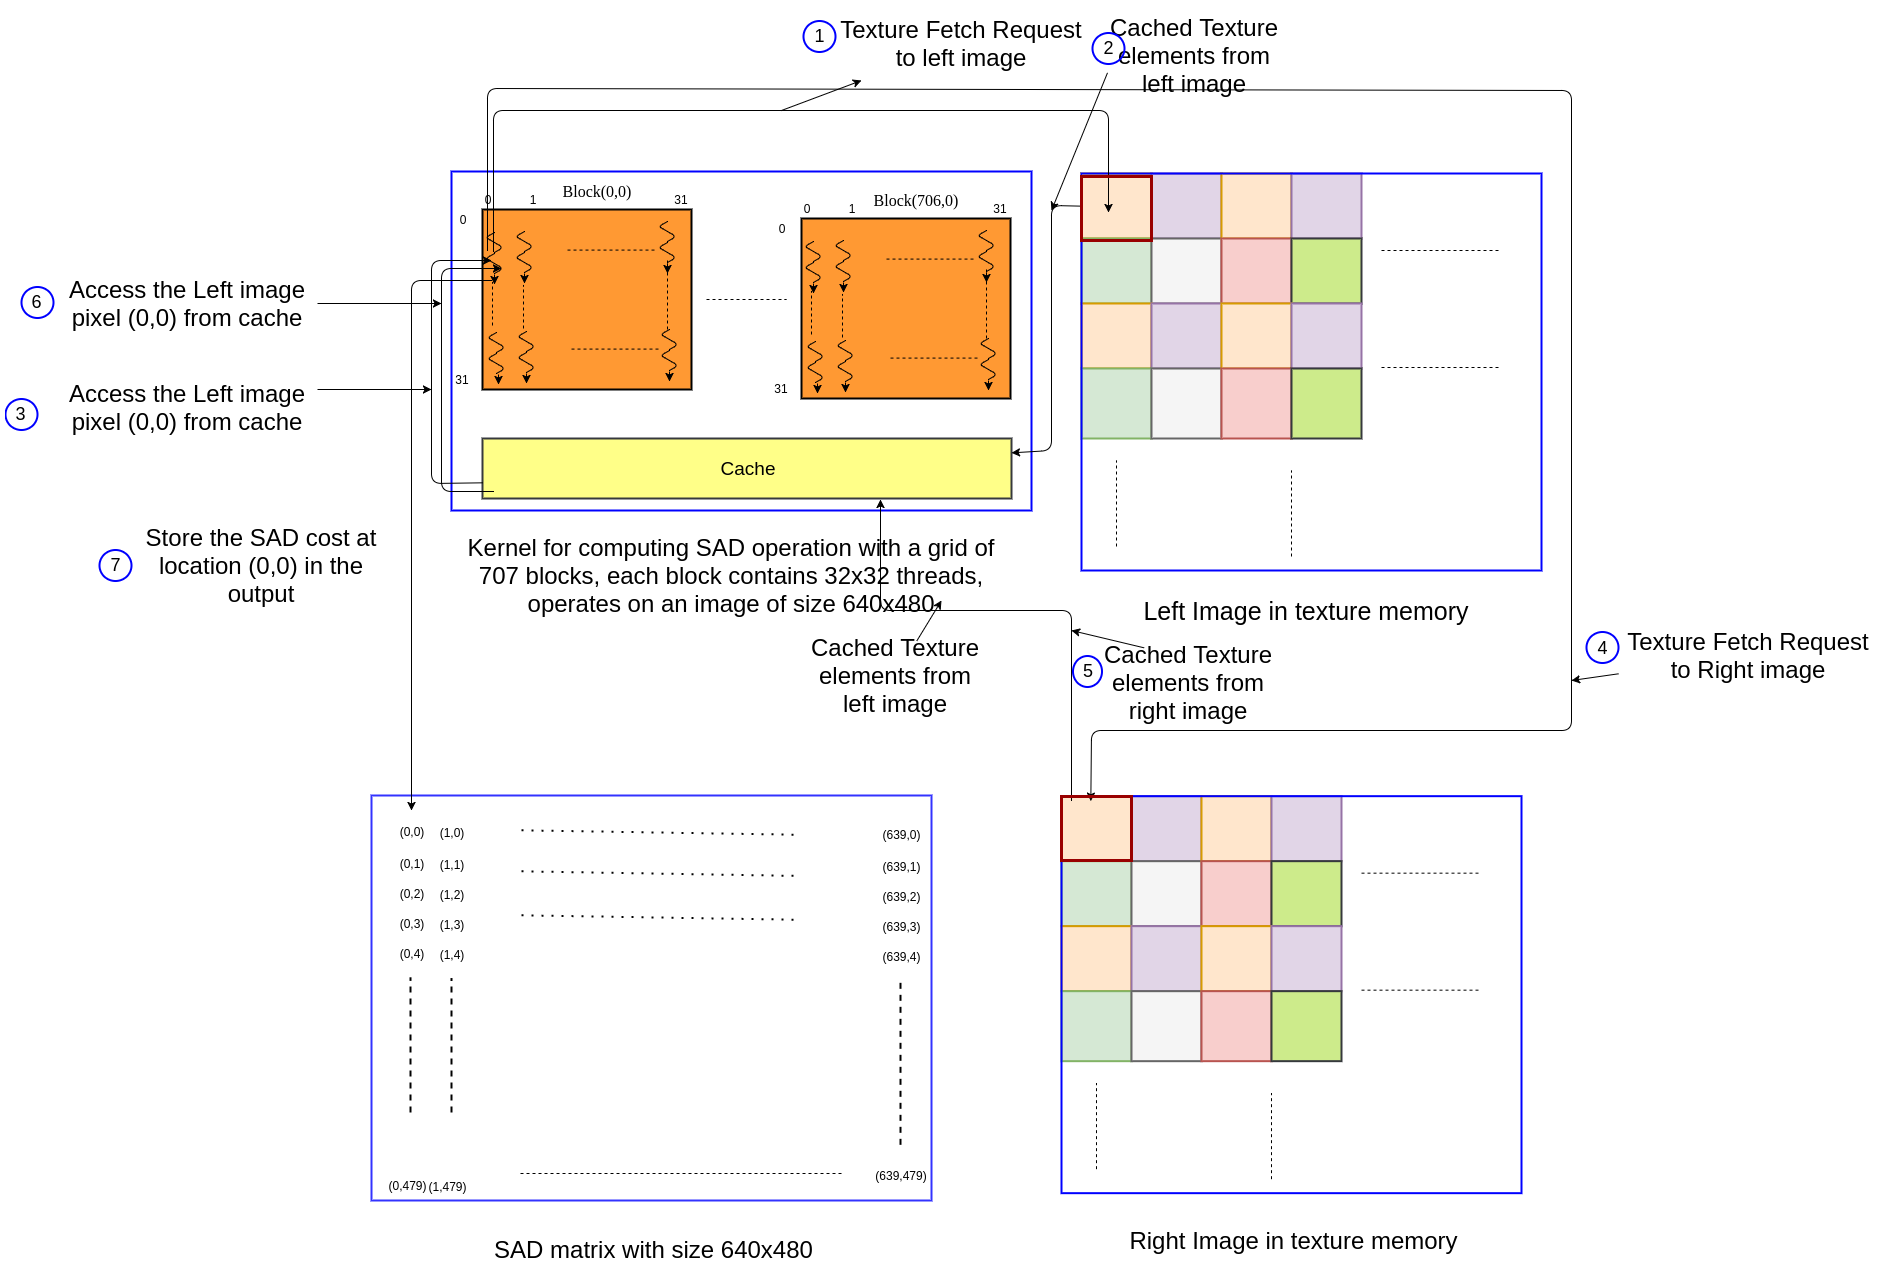
\includegraphics[width=1.2\linewidth]{textureMem.png}
				\caption{Texture memory usage for SAD kernel for an image of size 640x480}
				\label{fig:Texture}
			\end{figure}
	\end{itemize}
	\item CUDA intrinsics can be used to perform SAD operations very quickly in a single cycle.
	\begin{itemize}
		\item In general implementation like in the Equation \ref{SADeq} the difference is found for each component of the pixel. Here exist some parallelism using CUDA intrinsics, since each component takes a single byte to store, then CUDA per-byte intrinsics will do the difference operation to three components simultaneously and will add all the differences at the end to give a single value.
		\item This CUDA SAD intrinsics work on a 4 byte memory chunk. The three components in each pixel are packed as a single element with Alpha channel at the end. The alpha channel appended to each pixel will have zero value.
	\end{itemize}
	\begin{figure}[h!]
		\centering
		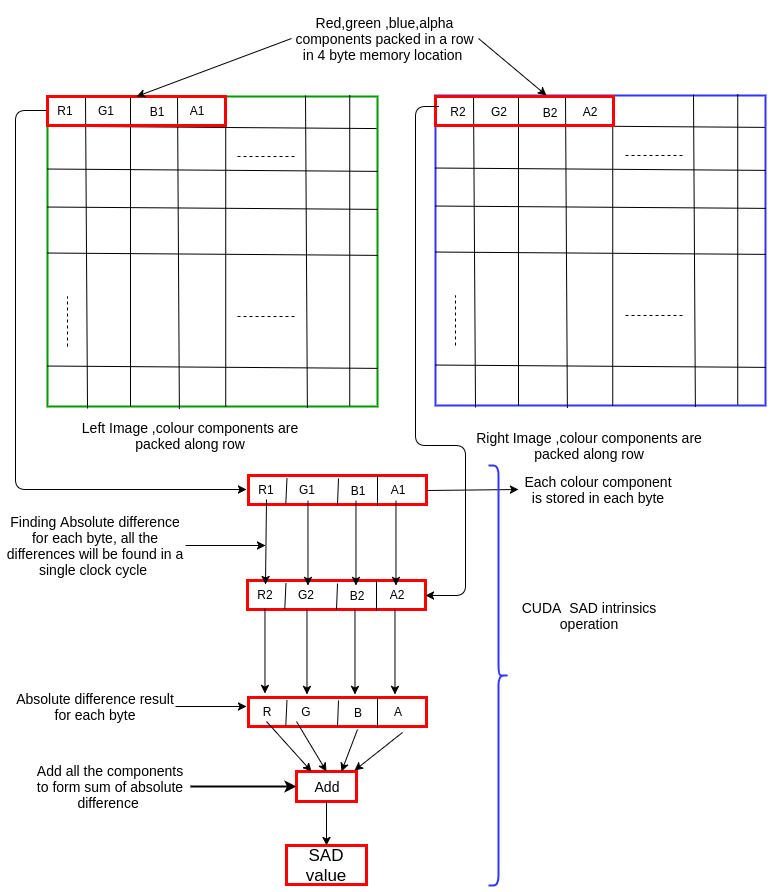
\includegraphics[width=\linewidth,height=12cm]{stereoDisparityCudaIntrinsics.png}
		\caption{CUDA SAD intrinsics operation}
		\label{fig:CUDA intrinsics}
	\end{figure}
	\item Parallel Streams can be used to Implement the independent operations concurrently in the algorithm, Finding the SAD costs for 17 disparity levels is qualified for streams based implementation.
	\begin{itemize}
		\item A stream ia a sequence operations that run on GPU in the order which CPU has issued. Operations in the streams can be run in parallel if sufficient device resoures are available for execution.
		\item The close observation on the above implementation reveals that the SAD matrices found in different pixel shifts of the reference image are independent of the other. So, all the SAD matrices can be found simultaneously using streams.
		\item Streams in CUDA can run different kernels simultaneously, with the limitation that the kernels shouldn’t exhaust the resources of the GPU.
		\item To implement the stereo disparity algorithm using streams, the number of resources used per each kernel are reduced, making kernels light weight. So that any single kernel will not exhaust the entire GPU resources.
		\item When modified for streams, the per thread load is increased such that each thread is given more work. The initial implementation creates 704 blocks with 1024 threads in each block, it occupies 90\% of the GPU resources. On the other hand created 8 blocks with 256 threads in each block, so that 4 threads works for each row of an image with size 640x533, the increased work load per thread decreased the occupancy to 13\% while increasing the time for execution of the kernel.
		\item The separable convolution implementations are also modified according to the streams. For these two kernels , image is processed patches wise. The horizontal separable convolution before modification creates a grid of 18x20 blocks with 32x32 threads in each block. And also, vertical separable convolution before modification creates a grid of 17x20 blocks with 32x32 threads in each block. Both the kernels use 90\% of the entire hardware individually. So, to run many of those kernels in parallel they are modified such that a grid of 4x4 blocks with 16x16 threads in each block are created, now the modified kernels takes each around 13.5\% of the resources.
		\begin{figure}[htb]
			\centering
			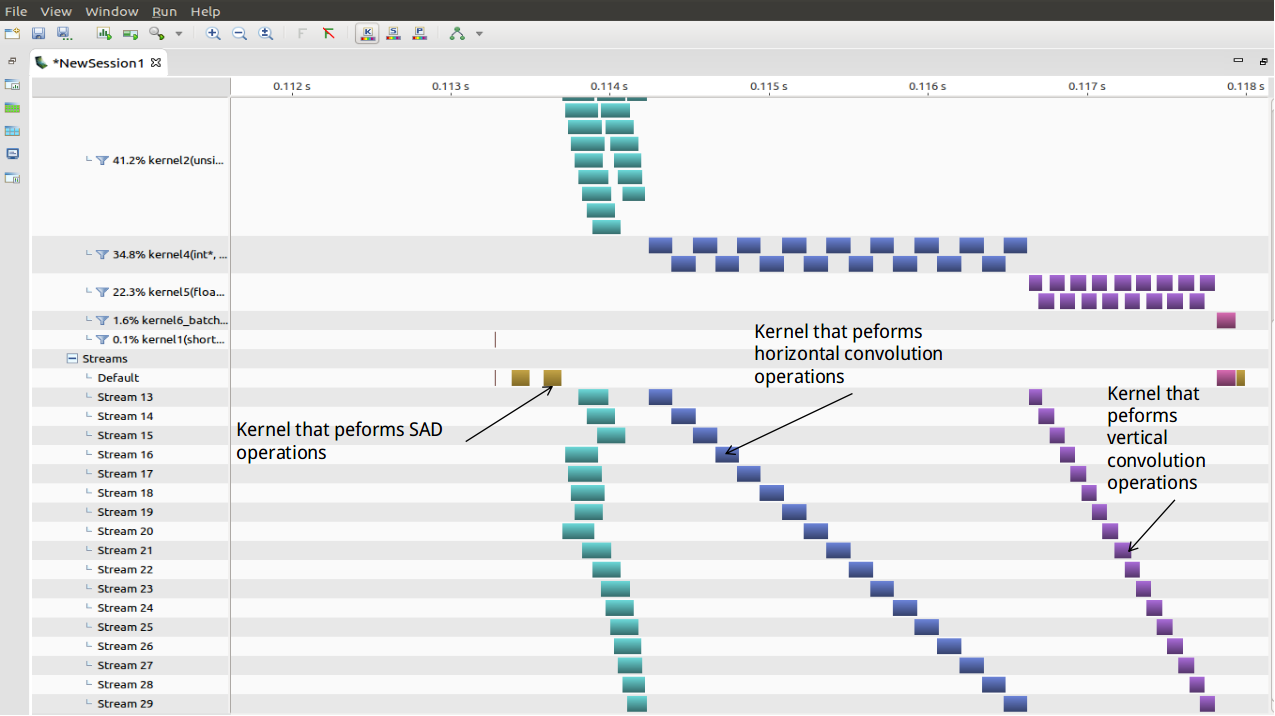
\includegraphics[width=\linewidth]{withoutConcurrency.png}
			\caption{NVIDIA Visual Profiler time-line for streams based implementation of stereo disparity blockmatching, kernels are without tweaking the thread-block configuration, working on an image of size 640x480}
			\label{fig:full occupancy}
		\end{figure}
		\item The Figure \ref{fig:full occupancy} shows the NVVP time-line for streams based implementation before reducing the occupancy of the kernels. The kernels are not light weight, so no concurrency is observed.
		\item The Figure \ref{fig:reduced occupancy} shows the NVVP time-line for stream based implementation after decreasing each kernel occupancy,  around 8 streams are able to run in parallel. Each kernel is tweaked so that they are consuming approximately 14\% of the SM resources.
		\begin{figure}[htb]
			\centering
			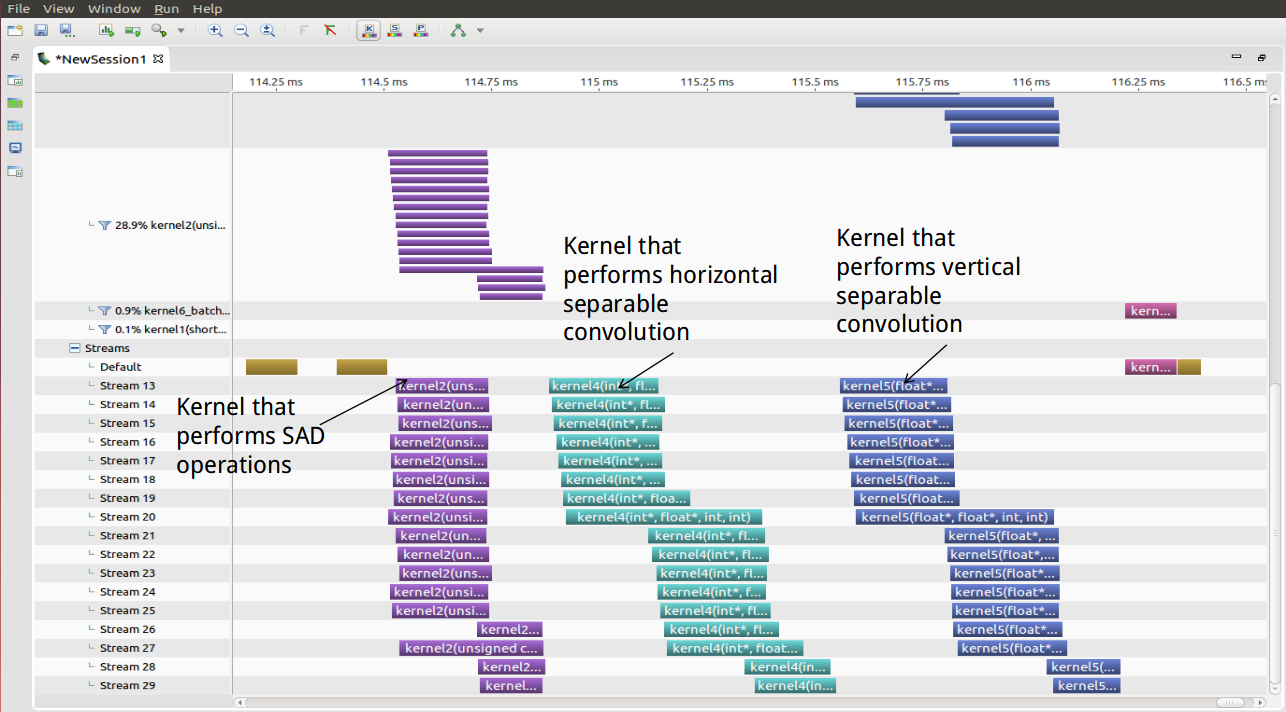
\includegraphics[width=\linewidth]{withconcurrency.png}
			\caption{NVIDIA Visual Profiler time-line for streams based implementation of stereo disparity block matching, kernels are tweaked such that the thread-block configuration is changed to reduce the occupancy, working on an image of size 640x480}
			\label{fig:reduced occupancy}
		\end{figure}
		\item The kernels in this streams implementation are not able to run concurrently on NVIDIA GT 640 and GTX 960, But on NVIDIA GTX 1070 GPU 8 kernels are able to run concurrently. Table \ref{fig:GPU resources} shows the mentioned GPU specifications.	
			\begin{table}[htb]
				\centering
					\resizebox{\columnwidth}{!}{%
				\begin{tabular}{|c|c|c|L|}
					\hline
					GPU & SM count & Core count per SM&Total cuda cores \\ \hline
					GT 640 &2&192&384 \\ \hline
					GTX 960&8&128&1024 \\ \hline
					GTX 1070&15&128&1920 \\ \hline
					Tegra X1 SoC intgrated GPU &2&128&256 \\ \hline
				\end{tabular}}
				\caption{Hardware resources of different GPUs used for stereo disparity block matching}%
				\label{fig:GPU resources}
			\end{table}
	\end{itemize}
\end{itemize}
		\subsection{Results and discussions}
		The stereo disparity block matching algorithm implementation is implemented on an NVIDIA GTX 1070 GPU. 
		The timing performance of the algorithm with streams and without streams implementations are tabulated in Table \ref{stereodisp with varied inp sizes}. From the Table \ref{stereodisp with varied inp sizes}, it is observed that a small performance gain is achieved with streams based implementation. This is due to the increased memory requests or hardware resource utilization bottleneck. The images in Figure \ref{fig:stereo disparity inputs} are input to the stereo disparity and the image in Figure \ref{fig:stereo disparity output} is the output of the algorithm.
		
		\begin{table}[h!]
			\centering
			\begin{tabular}{|c|c|L|L|}
				\hline
				\textbf{S.No}&\textbf{Image Resolution (Widthxheight)}&\multicolumn{2}{c|}{\textbf{\small Timing performance (in ms)}} \\ \cline{3-4}
				&&\scriptsize \textbf{Implementation without streams}&\scriptsize \textbf{Implementation with streams} \\ \hline
				1&320x240&1.75&2.3 \\ \hline
				2&640x533&4.7&4.68 \\ \hline
				3&800x600&6.14&5.6 \\ \hline
				4&960x720&7.5&6.8 \\ \hline
			\end{tabular}
			\caption{Stereo disparity performance on GeForce GTX 1070 for varied sizes of input image}%
			\label{stereodisp with varied inp sizes}
		\end{table}
		
	\begin{table}[h!]
			\centering
			\begin{tabular}{|c|c|L|}
				\hline
				\textbf{S.No}&\textbf{GPU model}&\textbf{\small Timing performance (in ms)} \\ \hline
				1&GeForce GT 640&24.8\\ \hline
				2&GeForce GTX 1070&4.7 \\ \hline
				3&Tegra X1 SoC intgrated GPU&45.6 \\ \hline
			\end{tabular}
				\caption{Stereo disparity performance on different NVIDIA GPUs for an image of size 640x533}%
				\label{stereodisp with varied GPUs}
	\end{table}
		\begin{figure}[h!]
			\centering
			\subfloat[Left]{{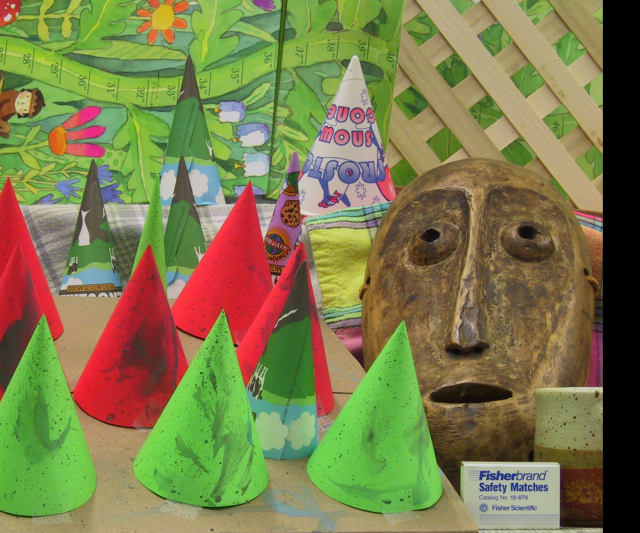
\includegraphics[width=6cm]{stereoDispInputLeft.png} }}%
			\qquad
			\subfloat[Right]{{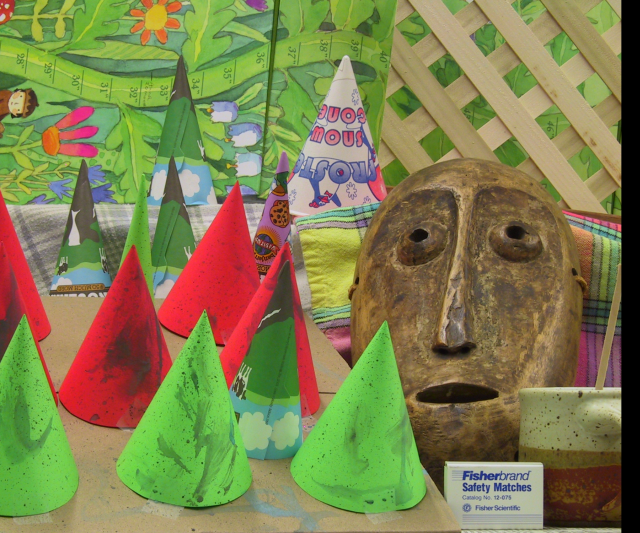
\includegraphics[width=6cm]{stereoDispInputRight.png} }}%
			\caption{Stereo disparity block matching algorithm inputs with size 533x640}%
			\label{fig:stereo disparity inputs}%og
		\end{figure}
	\begin{figure}[h!]
		\centering
		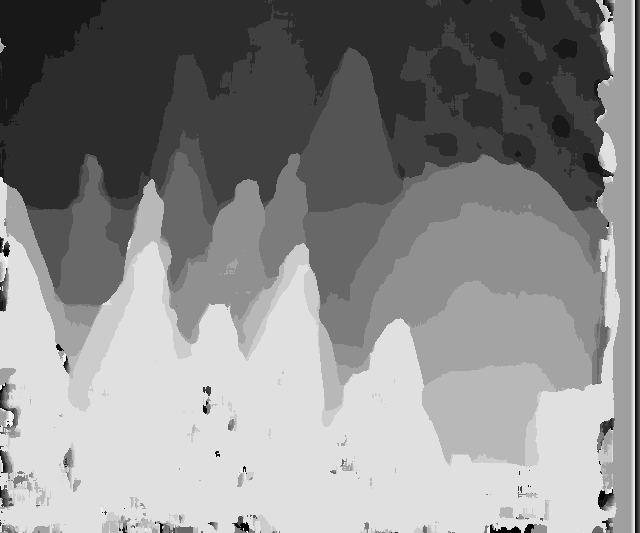
\includegraphics[width=0.6\linewidth]{stereoDispOutput.png}
		\caption{Stereo disparity output with size 640x533}
		\label{fig:stereo disparity output}
	\end{figure}
%\end{document}